\chapter{Background}
\index{Background@\emph{Background}}%is


\section{Phonetic Realization of Trochees in Spoken Verse} 


%In order to discuss questions regarding word-prosodic Estonian rhythm in the context of musical rhythm, I define the acoustic and perceptual notions of both domains, beginning with musical meter more generally, and continuing into the Estonian language and relevant verbal art forms. Once established, I then give a thorough overview of
% previous research in the domain of song and word prominence in Estonian {\it regilaul}. All this culminates into the research questions and hypotheses that are the subject of this paper. 
%\section{musical meter}
%
%
%
%
%\section{Estonian Word Prosody}
%
%
%
%The rhythmic organization of song integrates the prosodic structure of the language with musical rhythmic principles \citep{palmerLinguisticProsodyMusical1992}. 
%
%Duration can be a phonetic correlate of stress, and it can also be independently contrastive at the segmental level \citep{lehistePhoneticsMetrics1992}. 
%
%
%Whether there is a correlation between poetic metre and the prosodic structure of a language.
%
%A trochee is a strong, stressed syllable followed by a short(er), weak syllable. 
%
%
%
%
%\citep{lehistePhoneticsMetrics1992} investigated the actual phonetic realization of different metres in different languages, finding evidence for one language's trochee, for example, to be realized in a way that is systematically different from another language's trochee. 
%
%Ross found vowel reduction in certain notes, but they were all unstressed, off-ictus for that song\citep{rossFormants90}.
%
%
%The role of primary stress in Estonian is described by Ilse Lehiste as {\it identificational} rather than contrastive \citep{lehistePhoneticsMetrics1992}. In other words, there are no stress minimal pairs at the lexical level, so the prominence cue is to indicate the onset of a new word. This is sometimes also called {\it demarcative} stress.
%
%
%
%Three proposed levels of stress: primary stress, unstress, and secondary stress. \citep{lippusAcousticStudyEstonian2014a}
%
%Primary lexical stress in native Estonian words is fixed, falling on word-initial syllables. 
%\cite{eekmeisterUralica98}
%\begin{exe}
%\ex \gll laul-da \\
%	{[ˈlɑuːl.dɑ]} \\
%	sing-\Tr{} 
%	\glt	`singing'
%\ex 	ööbik \\
%	{[ˈøː.pikː]} \\
%	nightingale.\Nom{} 
%	\glt`nightingale'
%\end{exe}
%
%Estonian has three syllable weights, also called degrees or quantities, that are contrastive in primary stress position. The first degree or Q1 is described as short, 
%In \ref{quant_cont}, we see two minimal pairs illustrating this contrast. 
%
%This ternary contrast has long been the subject of debate in the phonological literature of metrics: Q3 syllables have been analyzed both as a monosyllabic foot \citep{princeMetricalTheoryEstonian1980} and as a trimoraic syllable \citep{hayesCompensatoryLengtheningMoraic1989, kuznetsovaEstonianWordProsody2018,prillopMoraeEstonianReply2020}. 
%
%
% \begin{table}[htb]
%\centering
%\begin{tabular}{lcc}
%\hline
%
%Q1 &		 sada 		& 	kabi  \\  
%	&	 {\it `hundred'} 	&	 {\it`hoof' }\\
%\hline
%Q2 &		saada 		&	kapi \\
%	&	 {\it`send' }		&	{\it`of the cupboard' }		\\
%\hline
%Q3 &		saada 	&	 kappi 	\\
%	&	{\it`recieve' }	&	{\it`into the cupboard' }	\\
%\hline
%\end{tabular}
%\label{qexamps}
%\caption{ternary syllable weight contrast}
%\end{table}
%
%
%Detail the acoustic-phonetic features of syllable weight and stress in spoken Estonian alongside the relevant findings from perception studies. 
% 
%
%
%
%
%
%Duration can be a phonetic correlate of stress, and it can also be independently contrastive at the segmental level \citep{lehistePhoneticsMetrics1992}. 
%
%
%only two quantity levels of syllables in monosyllables: function words (CV) are taken to be light, and lexical monosyllables (CV(V)C(C)) strong.
%
%\paragraph{INTO PROSE}
%domain of syllabic quantity is evident whre the first, stressed syllable increases in duration with increasing degree of quantity, the following unstressed syllable decreases. 
%Lehiste's duration ratios. 
%Different f0 patterns in Q2 and Q3: early peak, dramatic fall in 3, late peak and no fall in 2 (contradicts that asymmetry paper that still saw falls in all three... that could be related to the Q/A issue! Dang.)
%Laboratory speech usually confirms temporal and tonal characteristics, but conversational speech shows only duration (ratio) as stable, with Q3 fall often absent. 
%
%RQ: can quantities in conversational speech be distinguished by acoustics alone, or are listeners making use of semantic context. 
%
%disyllabic words from recorded conversational speech presented without context. 
%
%Q3: V1 durations had strongest influence on listener decisions, followed by f0 change within V1. duration ratio had a weaker influence, was only significant for stimuli of single speaker. f0 movement across intervo aclic consonant not significant in any case. similar results for recognition of Q3 when presented in combination.
%
%For combined Q1 and Q2, only duration of V1 significant across speakers, duration ratio only relevant for (same as earlier) speaker. 
%
%f0 peak position had no significant effect in the cases where it was present. 
%
%for good recognition of all three quantities, duration of first vowel important. 
%
%differences in V1 duration robust, even in changing speaking rate. ``characteristic" fall in f0 of Q3 neutralized. 
%
% listeners did not recognize the majority of Q3 syllables in the absence of context. 
% 
% certain minimum duration of V1 needed for high recog rate of Q3, 
% 
% these were all words that could change in meaning with degree of quantity,
%\citep{krullUralica98} 
%doctrine of ternary contrasts, lol 
%a: three contrastive segmental lengths
%b: segment structure {\it and} prosody of stressed syllable
%c: in the foot
%
%\par
%
%domain of prosodic patterns is the foot, but only the stucture of the primary stressed syllable is relevant in determining the Q degree of both syllable and foot. (i.e., there is no Q3 foot that does not contain a Q3 syllable as its initial.) 
%
%Q1 and Q2 must have at least two syllables, may have three (trochee, dactyl). Having a third syll does not effect quantity. This is in contrast to finnish trisyllables in folksongs, which were 40\% longer than disyllables. 
%
%Second syllable does not influence the quantity of the first. If the duration of second syllable is predictable from Q of first syllable, this is what phonologists refer to as dependent features. !!!RATIO ARGUMENT
%
%monosyllabic Q3 feet in succession in connected speech {\it `khev `kõhn `poiss `läks `kepp `käes; `tõu `suur `selts `kond `likkus}
%
%ratio theory initially proposed by Lauri Posti in 1950. 
%
%length of the vowel of the second syllable is redundant, dependent, and predictable. 
%
%Q3 is monosyllabic foot, making ``disyllables" technically trisyllables... 
%
%from segments toward long syllables is turning point, segments are a failure (lol) 
%\citep{hintUralic98}
%
%oot quantity paradigm
%short-long not separate phonological categories. long monophthongs behave like diphthongs, geminates as consonant clusters
%
%(in english, short and long vowels have different qualities: Wiik 1965
%
%(stressed syllables) Q3 largest area, Q1 most centralized in F1xF2 plane. 
%\par
%
%when f3 and f4 are removed from spectrum, /i/ is perceived as /ü/, /e/ as /ö/
%state that contrast twixt above two vowel pairs on basis of f3. authors say that f3 being close to the strong f2 in round-front is `amplified' the cumulative of f2 and f3.
%
%conclude perceptual param f2 describes well the perceptual phenom governing this contrast. 
%
%``effective" f2' values??
%calculate with: Bladon, Fant 1978: 3 
%
%long and short vary very little in quality, defining as different phonemes based on length is not justified. 
%
%Q3 more ``prototypical" or best-contrast version of vowel phonemes in space of stressed syll
%
%in unstress: 
%
%Q1 {\it least} central, unstressed following Q3 init most centralized. V in sylls following Q2 intermediate between others. (ok, they are analyzing these with the ``feet" as having the quantity.. 
%
%/i/ most resistant to centralization
%
%\citep{rossFormants90}
%REASON TO RE-EXAMINE VOWEL FORMANTS/SPACE IN  REGILAUL!!! 
%also, data to support ``vowel space" as an available acoustic modification (measurable) in 
%singing, evidence favors reduction in word-level-weak syllables AND off-ictus are reduced, 
%but to what extent, and how compared across ictus-stress and ictus-quantity?
%TLDR are vowels reduced in singing compared to speech, or were those vowels reduced compared with strong positions of song, of word? etc. 
%all these ``long" notes are off-ictus: so the shorter notes are corresponding to HEAVIER and STRONGER syllables. 
%singer's formant in untrained female voice very unlikely. measure: LTAS for /a/,/e/, /i/, /u/. SPL of peaks around 3kHz ~30-40dB less than that of the first formant in all four vowels. 
%
%
%
%HOWEVER all vowels selected were in off-ictus-- HUAT
%FIND THIS SONG NOW
%
%READING LIST: Rossing et al 1987- formant SPL in opera and choir singing: singer's formant usually closer to and sometimes converging on f1 SPL. 
%
%SAMEAUTHORSAMESONG: no significant timing differences between performers with respect to note durations (Ross 1989)
%*******Discussion similarity f3 in spoken and sung vowels 
%Ternström and Sundberg 1989: caution against using f3 and f4 standard deviations
%
%standard dev for third and fourth formants less vowel dependent, more ``personal," especially compared to standard dev of f2 and f2 f1 f2 which are {\it fairly} independent of subjects!!!
%
%
%inverse filter results to confirm T n S 87: f3 lower in singing? 
%saw some similar patterns in with spoken data studies, but overall the size of the variation was small. For the third formant, deviations of the sung vowels from spoken tend to be minor and irregular  n = 2
%
%overall f1/f2: sung vowels cluster compared to spoken, specifically:
%f1 raised in everything but /a/,
%f2 lower in front, raised in back. 
%
%So, gradient modification of vowel quality contrast (less different than in speech).. but I am getting an impression of a larger overall vowel space
%
%
%\subsection{syllable prominence}
%
%Three proposed levels of stress: primary stress, unstress, and secondary stress. \citep{lippusAcousticStudyEstonian2014a}
%
%Primary lexical stress in native Estonian words is fixed, falling on word-initial syllables. 
%\citep{eekmeisterUralica98}
%\begin{exe}
%\ex \gll laul-da \\
%	{[ˈlɑuːl.dɑ]} \\
%	sing-\Tr{} 
%	\glt	`singing'
%\ex 	ööbik \\
%	{[ˈøː.pikː]} \\
%	nightingale.\Nom{} 
%	\glt`nightingale'
%\end{exe}
%
%Some loanwords will allow primary stress to fall on a non-initial syllable: {\it example, example}. 
%Borrowed names occasionally shift stress to the typical Estonian position: for this reason one could find both {\it Maria} and {\it Maarja} in the same classroom. 
%
%The role of primary stress in Estonian is described by Ilse Lehiste as {\it identificational} rather than contrastive \citep{lehistePhoneticsMetrics1992}. In other words, there are no stress minimal pairs at the lexical level, so the prominence cue is to indicate the onset of a new word. This is sometimes also called {\it demarcative} stress.
%
%Spectral tilt suggested, but no
%\citep{sluijterSpectralBalanceAcoustic1996, lippusAcousticStudyEstonian2014a} \\
%
%
%\begin{table}
%\centering
%\begin{tabular}{lcccr}
%a & & & & u \\
%\end{tabular}
%\label{vowelinv} 
%\end{table}
%Vowels in this position are rarely reduced, and the full inventory of vowels is allowed. A total of 36 diphthongs are allowed in primary stressed positions. All nine vowels can be the first portion of a diphthong, but only [ɑ e i o u] appear as the second portion of the diphthong \citep{asuEstonian2009}. 
%
%\begin{itemize}
%\item diphthongs 
%\item example
%\end{itemize}
%
%
%Unstressed syllables, often have reduced vowels, and are more restricted in inventory: only three diphthongs [ɑi ei ui] are allowed in this position \citep{lippusAcousticStudyEstonian2014a}. 
%
%Examined the phonetic correlates of stress in Estonian, but it was small scale and dealt only with nasal flow, amplitude, and duration, and at multiple levels of prosodic hierarchy \citep{gordonPhoneticCorrelatesStress1997}, but with as few as two participants. 
%More recently and with more statistical power, researchers measured mean F0, standard deviation of F0, vowel duration, and spectral emphasis. They found increased vowel duration to be the most important acoustic correlate of primary stress in Estonian words, and that Unstressed syllables in Estonian have been documented to attract creaky voice \citep{lippusAcousticStudyEstonian2014a}. 
%Expound on this study a bit more
%Estonian facts \citep{alma991001659729706011} \\
%A pattern of secondary stress (neutral) has been attested, though phonetic evidence is limited \citep{asuAcousticCorrelatesSecondary2018}. Only initial and peninitial syllables are examined in the present study.
%
%studies on the perception of these contrasts to be inserted in prose: 
%
%\citep{meisterPerceptionShortVs2011a, kaskPerceptualAsymmetriesAuditory2021, eekSimplePerceptionExperiments1997}
%
%
%\subsection{syllable quantity}
%Primary stress position is where the well-known ternary syllable weight contrast in Estonian appears.
%
%
%About this section: flows well, contains good information. Needs a little more information, as indicated below.
%Missing in this section: there's no discussion of what syllable weight/quantity means, either generally or in relation to Estonian. We represent syllable in terms of moras. What would the moaic representations for Q1, Q2, and Q3 be? Your designations short, long and overlong aren't specific enough and it's ot clear what the basis for the ratio is.
%
%
%Estonian has three syllable weights, also called degrees or quantities, that are contrastive in primary stress position. The first degree or Q1 is described as short, 
%In \ref{quant_cont}, we see two minimal pairs illustrating this contrast. 
%
%This ternary contrast has long been the subject of debate in the phonological literature of metrics: Q3 syllables have been analyzed both as a monosyllabic foot \citep{princeMetricalTheoryEstonian1980} and as a trimoraic syllable \citep{hayesCompensatoryLengtheningMoraic1989, kuznetsovaEstonianWordProsody2018,prillopMoraeEstonianReply2020}. 
%
%
%
%
% \begin{figure}[htb]
% \begin{center}
% 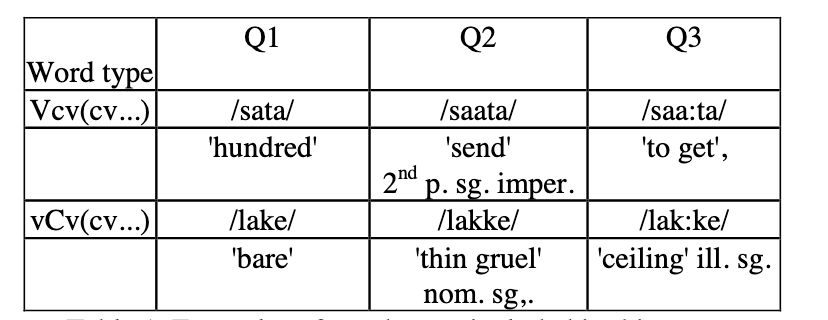
\includegraphics[width=200pt]{figures/Quantity.png}\\
%
% \caption{Ternary Quantity Contrast {\citep{krullFOOTISOCHRONYESTONIAN1999}}}
% \label{quant_cont}
% \end{center}
% \end{figure}
%
% \begin{table}[htb]
%\centering
%\begin{tabular}{lcc}
%\hline
%
%Q1 &		 sada 		& 	kabi  \\  
%	&	 {\it `hundred'} 	&	 {\it`hoof' }\\
%\hline
%Q2 &		saada 		&	kapi \\
%	&	 {\it`send' }		&	{\it`of the cupboard' }		\\
%\hline
%Q3 &		saada 	&	 kappi 	\\
%	&	{\it`recieve' }	&	{\it`into the cupboard' }	\\
%\hline
%\end{tabular}
%\label{qexamps}
%\caption{ternary syllable weight contrast}
%\end{table}
%
%
%\gll valge lauade vahele, \\
%white boards between \\
%\glt in between white boards, \\
% 
%Syllable weight or quantity also influences the otherwise predictable stress pattern. When a Q3 syllable is not in the first position, primary stress falls on it: this usually happens in the case of borrowed words. Otherwise, primary word stress is on the first syllable \citep{lehisteFunctionQuantityFinnish1965}. 
%  
%  \begin{table}[htb]
%\centering
%\begin{tabular}{lcr}
%\hline
% 	 Q1 – short 	&	ratio ~2/3 \\
%	 Q2 – long		& 	ratio ~3/2	\\
%	 Q3 – overlong	&	ratio ~2/1 	\\
%	 \hline
%\end{tabular}
%\label{stressick}
%\caption{c}
%\end{table}
%
%In the initial syllable of a word, syllable duration increases with syllable quantity, while the second syllable in the foot decreases as the first syllable's quantity increases. 
%
%It has been suggested, that the duration of the second vowel is a diagnostic of the quantity of the preceding syllable (duration ratios) \citep{lehisteFunctionQuantityFinnish1965, lehisteProsodicChangeProgress2003}. It has been suggested that this is due to the 
%a documented tendency for foot isochrony, wherein the total duration of disyllabic feet varies little in both spontaneous and read speech \citep{krullFOOTISOCHRONYESTONIAN1999, traunmullerEffectLocalSpeaking2003}resulting in the inverse relationship between the durations of the two syllables in a foot: the longer the first syllable, the shorter the second. More specifically: a second syllable that follow an overlong syllable will be realized shorter than a second syllable that follows a long syllable, with the longest second syllables following short (Q1) first syllables.  
%%\footnote{further discussion of perception of ternary quantity and duration ratios to put into prose \citep{foxDiscriminationDurationRatios1987,foxDiscriminationDurationRatios1989}}
%
%
%Duration ratios, but all proportionally 50\% differences. The ``long" second syllable of Q1 is shorter still than the ``short" second syllables of Q2 and Q3 feet. 
%\citep{lehiste1960segmental}
%\subsection{perception of word prosody}
%
%
%
%
%suggested analysis as types of foot accents rather than syllable degrees. 
%rising or falling f0 alone was insufficient to change the perceived category of all three weights.
%lengthening V2 of third quantity, but maintaining its reduction, did not suffice to change the perceived cat of A3 to A2: only when the tone contour also changed to rising did the nucleus duration facilitate. 
%reducing quality and shortening duration of nucleus V2 of an A2 alone also did not change perception to A3: only when falling tone added.
%\citep{eekSimplePerceptionExperiments1997}
%
%
%
%
%foot isochrony resulting in inversely proportional duration ratios of S1:S2 syllables, or more plainly that as S1 increases in quantity, S2 nucleus decreases. \citep{eekSimplePerceptionExperiments1997}
%
%Q3 vowels described as having especially large standard deviations \citep{eek1975}. 
%
%\section{Emphasis in Songs}
%\subsection{strong beats}
%
%\section{Template for {\it runosong}} 
%Kalevala and regilaul 
%\citep{sarv1998language}\\
%The singing of folksongs has long been an important part of the Estonian national heritage, and large scale community gathering to sing traditional {\it regilaul} songs is argued to have aided the preservation of Estonian cultural and linguistic heritage through long periods of occupation. \citep{bruggemannSingingOneselfNation2014}. The first documented song festival in Estonia was held in the seventeenth century \citep{ruutelTRADITIONALMUSICESTONIA2004}.
%
%Most descriptions of {\it regilaul} will describe it as ``non-western" folk music, though the definition of western escapes the author. It is perhaps the reduced use of tempered scale, although the songs have distinct tonal centers, and the melodies rise and fall in intervals from it.  The ``non-western" ness could equally be the lack of ``end-rhyming," a signature innovation in newer Estonian songs, as traditional {\it regilaul} rhymes little in favor of alliteration and parallelism. If you listen to them, though, even completely naive of the Estonian language, you will not mistake them for anything but a folksong, and a strictly structured one at that. 
%
%A song called {\it regilaul} is a type of Estonian folksong, found within the greater songwriting tradition of Balto-Finnic language family: variations on these songs are found in Finnish, Karelian, Votic, and Ingrian traditions \citep{tormisKalevalaEstonianPerspective1985}. 
%
%Collectively, songs in this tradition are often referred to as ``runosongs" or ``runic songs." 
%
%These runic songs are set in what scholars refer to as The ``Kalevala" metre, named for the title of the epic poem in Finnish; Estonia's own version is called ``Kalevipoeg" {\it Kalev's son}. 
%
%In the story, Kalevipoeg is a giant with a hedgehog for a companion. 
%
%The poem contains songs, too: a consistent theme across these poems and Estonian folklore generally has protagonists requesting song lyrics and incantations from deities, often in pursuit of skill in dance or music. 
%
%In studies of metre, a trochee is a disyllabic sequence with a strong first syllable and a weak second. In {\it regilaul} songs, the strong position of a two note sequence is called ``ictus," and the weak position is called ``off-ictus"
%
% The basic template of the Kalevala metre is four trochees per line, for a total of eight syllables. There are of course variations, but the basic invariant {\it regilaul} verse line will contain eight beats evenly divided into a single measure: in a 4/4 song, each of the eight syllables corresponds with one eighth note. In this case each eighth note will correspond to one syllable in the text, the constituent henceforth referred to as the ``syllable-note" \citep{ruutelResultsComputerizedComparative1999}. The late composer and {\it regilaul} revitalist Veljo Tormis referred to the runic songs as ``singable songs" \citep{tormisProblemsThatRegilaul2007}. 
% 
% ``collaborative outcomes" 
% in regilaul, the musical rhythm is directly connected to the verse structure \citep{orasMusicalManifestationsTextual2010}
% 
% Due to the strict metrical parametres of the form, any runosong text can be sung to any runosong melody. An example of this in English: one can sing {\it Amazing Grace} to the tune of {\it House of the Rising Sun}, and vice a versa.\footnote{Also try TLC's ``Scrubs" exchanged with America's ``Horse With No Name"}. 
%\begin{figure}[htb]
%\begin{center}
%
\includegraphics[width=300pt]{figures/069.png}
%\caption{Öised orjad, performed by Liisu Orik}
%\label{song69}
%\end{center}
%\end{figure}
%
%In \ref{song69}, we see the musical notation of a typical {\it regilaul} verse: eight notes evenly divided into a measure (eight eighth notes) and corresponding one syllable per eighth note as indicated by the text. The refrain {\it kas`-ke}, which is repeated after every verse line, is part of a separate musical phrase, though it is not a full measure on its own (it contains only three beats). This is indicated by the dashed line following the first measure of the verse. The solid bar after the {\it kas`-ke} refrain indicates the onset of a new ``regular" measure, another {\it regilaul} verse line of eight syllables evenly divided into eighth notes in the measure. 
%
%\begin{figure}[htb]
%\begin{center}
%
\includegraphics[width=300pt]{figures/094.png}
%\caption{`The King Game" as performed by Liisa Kümmel on track 94 of the anthology}
%\label{kinggame}
%\end{center}
%\end{figure}
%
%In \ref{kinggame} we see an example of extra syllables fit into the Kalevala metre. The first measure in the figure is another refrain. Looking at the verse annotation, we see that there are in fact nine syllables instead of the requisite eight. The measure accomodates the extra syllable by dividing one of the eighth notes into two sixteenths. Thus, the one to one ratio of syllable to note remains, but only seven of the syllable-notes are annotated as isochronous. 
%
%Only those syllable-notes which are in evenly divided verse measures are the subject of this study. Non-verse notes, such as those in refrains, as well as notes in verses that occupy a different categorical duration than other notes in its measure are not included. 
%
%
%The composer Veljo Tormis refers to folksongs in this tradition as ``singable song," 
%
%shared structure of other Finno-Ugric language family, i.e., %
%%
%the singable song 
%
%
% ancient epic tale shared by many members of the Finno-Ugric language family
% 
% The common folklore of Finno Ugric language family: Kalavala in Finland, Kalevipoeg (Kalev's son) in Estonia. Kalev is a giant. His companion is a hedgehog.  
% many stories involve a character seeking incantations (song lyrics) to acquire some skill
% 
%
%
%\subsection{Previous phonetic studies of Estonian metrics and {\it regilaul}}
%
% \citep{palmerLinguisticProsodyMusical1992} hypothesize that prosodic stress and musical metre align in song, but their measurements were only of English vocalists and ``western" music. 
%English vocalists were asked to perform songs in which stressed syllables aligned or clashed with the musical meter, finding relative increases in syllable duration in at both word-level and song-level positions of prominence \citep{palmerLinguisticProsodyMusical1992}, suggesting that the two systems contribute separately but use similar organizational properties.
%
%Ilse Lehiste analyzed spoken poems in Estonian and Finnish, examining the differences in quantity relations under metrical subjugation and found that in strict metrical forms (i.e., the Kalevala metre), the absolute durations of Q2 and Q3 metrical feet lost their contrast, but retained the approximate ratio of durations between the first and second syllable. In freer verse, the differences in absolute durations remained, suggesting that the duration ration between Q2 and Q3 is an important cue for contrast, especially in the contexts of temporal demands of an imposed paralinguistic metre. 
%\citep{lehistePhoneticsMetrics1992} Later, in collaboration with Jaan Ross, three papers examined the phonetics of metrics in old Estonian {\it regilaul} folksongs. The first (Funeral laments study )\citep{rossLostProsodicOppositions1994}, finding that duration was best predicted by metrical position and not syllable quantity. 
%
%
%
%
%They later found that duration was a better predictor of ictus  than of word stress: stressed syllables in off-ictus lost their durational contrast with unstressed syllables.  \citep{rossTradeoffQuantityStress1996} 
%
%In \citep{rossTimingEstonianFolk1998} Ross and Lehiste measure syllable duration ratios for Q1 initial syllables of disyllabic feet: falling in ictus position and falling in off-ctus position. They found that the duration ratios of Q1 syllables in ictus were greater than those in off-ictus. In ictus position, Q1 syllables were roughly the same length as each other, while those in off-ictus were shortened. They conclude the duration cue for contrastive stress is subordinated to the song. 
%This paper aims to extend the findings of the aforementioned studies \citep{lehistePhoneticsMetrics1992, rossLostProsodicOppositions1994,rossTradeoffQuantityStress1996,rossTimingEstonianFolk1998} by annotating a larger corpus of {\it regilaul}, to compare conflicts of song stress (ictus) and word stress 
%and investigate whether syllable quantity contrast is preserved in song. Vowel duration is an acoustic correlate of both syllable stress and quantity, and so I measure vowel duration in the context of performed {\it regilaul} songs. 
%
%Vowel duration, if subordinated to the metre of the song, would confirm Ross \& Lehiste's results \citep{rossLostProsodicOppositions1994, rossTimingEstonianFolk1998, rossTradeoffQuantityStress1996}. 
%
%If this question has already been investigated, what motivates the author to pursue it further? First, the aforementioned studies were limited in sample size: each one examined only one word-level interaction with song-level prominence, when both are well documented to influence duration in spoken Estonian, and with each other. Thus, the present study examines all three predictors of prominence: song ictus, word stress, and syllable quantity. I also exponentially increase the {\it n} of trials for increased robustness, and then analyze the dataset using Bayesian modeling techniques to capture the nuanced covariance of the three predictor categories. In addition to replicating duration measurements undertaken in earlier studies, I also introduce vowel space as a potential predictor for word-level prominence. 
%
%more recently, text setting in regilaul
%\citep{orasMusicalManifestationsTextual2010}
%
%
%
%
%A good deal of literature has been devoted to the classification of languages by typological rhythms: in particular, ``stress-timed," ``syllable-timed," and ``morae-timed" systems have been proposed. An extremely reductionist description of these typologies would assert a relative isochrony of the named constituent. That is, a language that has been described as ``stress-timed" is said to be "timed" according to, and having relative isochrony of stressed syllables. Likewise, a syllable-timed language would be described as having syllabic isochrony, and so on. Many of these notions are based on the intuitions of native speakers, however, supporting phonetic data is limited  \citep{kohlerRhythmSpeechLanguage2009}. 
%%add later!!: (Bertinetto 1989) (Kohler 2009a, b). 
%More recently, alternate rhythmic metrics have entered the discussion in support of timing classes: i.e., Pairwise Variability Index (PVI), normalized Pairwise Variability Index (nPVI), both of which use the relationship of durations of adjacent syllables to describe their timing classes.\citep{arvanitiRhythmClassesSpeech2012}. English, for example, has higher syllable PVI (Pairwise Variability Index) than Estonian, due to English's drastic reduction of weak syllables, and the presence of prominent short syllables ( i.e., syllable durations in English are more variable than in Estonian)\citep{asuEstonianEnglishRhythm2006}. 
%
%
% 
% 
%\begin{itemize}
%\item is stress or ictus a better predictor of vowel duration?
%\item is the ternary syllable quantity contrast preserved in {\it regilaul} songs?
%\end{itemize} 
%
%\subsection{Design of the Study}
%
%Measurements:
%
%vowel duration
%
%vowel dispersion
%
%stressed syllable less reduced, more intelligible, 
%
%Fine-grained acoustic-phonetic cues to stress (cross-linguistic) 
%\citep{lindblom1990,moonInteractionDurationContext1994, de1995supraglottal, bradlowIntelligibilityNormalSpeech1996,smiljanicProductionPerceptionClear2005} \\
%\subsection{On foot isochrony and duration ratios} 
%
%However, in both cases, the presence of foot isochrony and consistent duration ratios across these three types of feet would not indicate that the foot is the domain of the contrast, nor that the ratio itself is the measurement of importance. Instead, these two findings point to the level of contrast between Q1, Q2, and Q3 syllables at the level of the syllable, and the resulting fluctuations in ratios of first and second syllables as inevitable consequences of preserving the contrast in initial position. 
%
%Another consideration is that the three quantities are not restricted to length contrasts of identical segments, in the case of the geminates seen in minimal triads, but also can be comprised of diphthongs and complex codas {\it in addition} to geminates. 
%, i.e., ui: (diphthong ending in long V), diphthong complex coda geminate consonant, etc. \\ 
%
%
%contain more phoneme segments. The minimal triads illustrate the segmental length contrasts that provide evidence for the three weights of syllables in primary stress position, but they do not adequately convey that the different quantities are not simply different lengths of segments, but that with an increase syllable quantity comes an increase in the quantity of segments contained within that constituent. To illustrate this, the table in \ref{} contains representations of available segment combinations in each syllable, and examples of Estonian near-minimal triads in disyllabic words. 
%
